%%%%%%%%%%%%%%%%%%%%%%%%%%%%%%%%
%%% 課題II
%%%%%%%%%%%%%%%%%%%%%%%%%%%%%%%%

\homework

%%%%%%%%%%%%%%%%%%%%%%%%%%%%%%%%
%%% II-1
%%%%%%%%%%%%%%%%%%%%%%%%%%%%%%%%

\question{
	テキストの図6に展開図を示す正四面体ABCD
	\footnote{本報告書では原点$\mathrm{O}$から$\bm{a}$にある点を$\mathrm{A}$と表記する.}
	について,$\triangle$BCDの重心Gを原点Oと一致させ,
	正四面体の一辺の長さを$w$とするとき,各頂点の3次元座標を導出せよ.
}

% 文章

$\triangle$BCDの高さは一辺が$w$の正三角形なので,$\sqrt{3}w/2$となる.
$\triangle$GBDが二等辺三角形となる.三平方の定理を用いて
$\triangle$GBDの等辺の長さは$w/\sqrt{3}$となる.
これらのことから正四面体の高さは三平方の定理を用いて,$\sqrt{2/3}w$となる.
よって各頂点の位置は次となる.
\begin{align*}
	\bm{a} &= \left(\sqrt{\frac{2}{3}}w, 0, 0\right) &
	\bm{b} &= \left(0, \frac{w}{\sqrt{3}}, 0\right) &
	\bm{c} &= \left(0, -\frac{w}{2\sqrt{3}}, \frac{w}{2}\right) &
	\bm{d} &= \left(0, -\frac{w}{2\sqrt{3}}, -\frac{w}{2}\right)
\end{align*}

% 図

\begin{figure}[htbp]
	\centering
	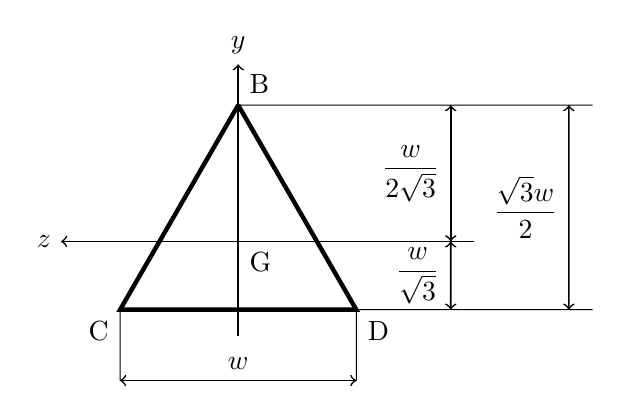
\begin{tikzpicture}[xscale=-3, yscale=3, ultra thick]
	%原点
	\draw (0, 0) node [below right]{G};
	%y軸
	\draw[semithick, ->] (0, -0.4)--(0, 0.75) node [above]{$y$};
	%z軸
	\draw[semithick, ->] (-1, 0)--(0.75, 0) node [left]{$z$};
	%頂点
	\path (0, 0.577) coordinate (B);
	\path (0.5, -0.289) coordinate (C);
	\path (-0.5, -0.289) coordinate (D);
	\draw (B) node [above right]{B};
	\draw (C) node [below left]{C};
	\draw (D) node [below right]{D};
	%辺
	\draw (B)--(C)--(D)--(B);
	%大きさ
	%
	\path (C)++(0, -0.3) coordinate (Cb);
	\draw[thin] (C)--(Cb);
	\path (D)++(0, -0.3) coordinate (Db);
	\draw[thin] (D)--(Db);
	\draw[semithick, <->] (Cb)--(Db);
	\draw (0, -0.589) node [above]{$w$};
	%
	\path (D)++(-0.4, 0) coordinate (Dr);
	\path (Dr)++(0, 0.289) coordinate (Or);
	\path (Dr)++(0, 0.866) coordinate (Br);
	\draw[semithick, <->] (Dr)--(Or);
	\draw[semithick, <->] (Or)--(Br);
	\path (Dr)++(0, 0.144) node [left]{$\displaystyle\frac{w}{\sqrt{3}}$};
	\path (Dr)++(0, 0.577) node [left]{$\displaystyle\frac{w}{2\sqrt{3}}$};
	%
	\path (D)++(-0.9, 0) coordinate (Drr);
	\path (Drr)++(0, 0.866) coordinate (Brr);
	\draw[semithick, <->] (Drr)--(Brr);
	\path (Drr)++(0, 0.433) node [left]{$\displaystyle\frac{\sqrt{3}w}{2}$};
	%
	\path (D)++(-1, 0) coordinate (Drrr);
	\path (Drrr)++(0, 0.866) coordinate (Brrr);
	\draw[thin] (D)--(Drrr);
	\draw[thin] (B)--(Brrr);
\end{tikzpicture}

	\hspace{4\zw}
	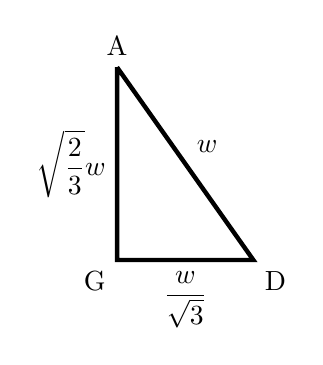
\begin{tikzpicture}[xscale=3, yscale=3, ultra thick]
	%頂点
	\path (0, 0.816) coordinate (A);
	\path (0, 0) coordinate (G);
	\path (0.577, 0) coordinate (D);
	\draw (A) node [above]{A};
	\draw (G) node [below left]{G};
	\draw (D) node [below right]{D};
	%辺
	\draw (A)--(G)--(D)--(A);
	%大きさ
	%
	\path (0, 0.408) node [left]{$\displaystyle\sqrt{\frac{2}{3}}w$};
	\path (0.289, 0) node [below]{$\displaystyle\frac{w}{\sqrt{3}}$};
	\path (0.289, 0.408) node [above right]{$\displaystyle w$};
\end{tikzpicture}

	\caption{正四面体の一部の大きさ}
	\label{fig:hw2-1}
\end{figure}

%%%%%%%%%%%%%%%%%%%%%%%%%%%%%%%%
%%% II-2
%%%%%%%%%%%%%%%%%%%%%%%%%%%%%%%%

\question{
	前問で求めた結果をもとに,原点Oを中心とする半径$1$の球に
	内接する正四面体の頂点がテキストのリスト14のように定まることを導出せよ.
}

% 文章

正四面体の重心$\bm{g}'$が原点と一致させるために前問の正四面体を移動させる.
重心$\bm{g}'$は,
\begin{align*}
	\bm{g}' = \frac{\bm{a} + \bm{b} + \bm{c} + \bm{d}}{4}
	= \left(\frac{1}{4}\sqrt{\frac{2}{3}}w, 0, 0\right)
\end{align*}
移動後の各頂点を$\bm{a}'$,$\bm{b}'$,$\bm{c}'$,$\bm{d}'$とすると各頂点の位置は,
\begin{align*}
	\bm{a}' &= \bm{a} - \bm{g}'
	= \left(\frac{1}{2}\sqrt{\frac{3}{2}}w, 0, 0\right) &
	\bm{b}' &= \bm{b} - \bm{g}'
	= \left(-\frac{1}{4}\sqrt{\frac{2}{3}}w, \frac{w}{\sqrt{3}}, 0\right)\\
	\bm{c}' &= \bm{c} - \bm{g}'
	= \left(-\frac{1}{4}\sqrt{\frac{2}{3}}w, -\frac{w}{2\sqrt{3}}, \frac{w}{2}\right) &
	\bm{d}' &= \bm{d} - \bm{g}'
	= \left(-\frac{1}{4}\sqrt{\frac{2}{3}}w, -\frac{w}{2\sqrt{3}}, -\frac{w}{2}\right)
\end{align*}
半径$1$の球に内接するとき$\bm{a}'=(1,0,0)$となるので$w=2\sqrt{2/3}$となる.
よって各頂点の位置は,
\begin{align*}
	\bm{a}' &= \left(1, 0, 0\right) &
	\bm{b}' &= \left(-\frac{1}{3}, \frac{2\sqrt{2}}{3}, 0\right) &
	\bm{c}' &= \left(-\frac{1}{3}, -\frac{\sqrt{2}}{3}, \frac{\sqrt{6}}{3}\right) &
	\bm{d}' &= \left(-\frac{1}{3}, -\frac{\sqrt{2}}{3}, -\frac{\sqrt{6}}{3}\right)
\end{align*}
この位置から各頂点の値がテキストのリスト14のように定まることがわかる.

%%%%%%%%%%%%%%%%%%%%%%%%%%%%%%%%
%%% II-3
%%%%%%%%%%%%%%%%%%%%%%%%%%%%%%%%

\question{
	テキストの\textbf{9.2}のアームロボットについて,キー入力で台座の回転と,
	各関節の傾斜角を制御できるような対話プログラムを作成してみよう.
}

% 文章

アームロボットの各パーツの登録部分を\Lstref{lst:hw2-3-1}に示す.
ここでは台座,下腕,上腕の登録をしている.
\footnote{
	\texttt{ID\_X}や\texttt{HEIGHT\_X}などは
	テキストのリスト27のようにマクロ定義してある.
}
キーボードコールバック関数を\Lstref{lst:hw2-3-2}に示す.
押されたキーに対応したパーツの角度を変え再描画している.
そして,テキストのリスト20と同様の関数\texttt{display}を用いて
アームロボットを描画する.

% リスト

\lstinputlisting[
	caption = 各パーツの登録(\texttt{init}の一部),
	label = lst:hw2-3-1,
	linerange = {14-14, 66-71, 73-81, 83-90, 92-100}
]{
	../../Homework/2/hw2-3.c
}
\lstinputlisting[
	caption = キーボードコールバック関数(\texttt{keyin}),
	label = lst:hw2-3-2,
	linerange = {13-13, 51-61, 63-65}
]{
	../../Homework/2/hw2-3.c
}

%%%%%%%%%%%%%%%%%%%%%%%%%%%%%%%%
%%% II-4
%%%%%%%%%%%%%%%%%%%%%%%%%%%%%%%%

\question{
	タイマーコールバックを使って,アームロボットを制御するようなプログラムを作成してみよう.
	アームロボットが踊っているかのように見せるには,どんな工夫ができるだろう.
}

% 踊ってるように見せるために

\subquestion{踊ってるように見せるために}

下腕と上腕を滑らかに手を振っているようにするには
各角度$\theta_{\mathrm{L}}$,$\theta_{\mathrm{U}}$を
\Equref{equ:theta-L},\Equref{equ:theta-U}とすることでできると考えた.(時刻を$t$とする.)
\begin{align}
	\theta_{\mathrm{L}} &= A\sin[B\sin(2t)]\label{equ:theta-L}\\
	\theta_{\mathrm{U}} &= A\sin[2B\sin(2t)]\;\;\;\;(AとBは任意定数)\label{equ:theta-U}
\end{align}
$A$と$B$を変えることで動きの速さを変えることができる.
下腕と上腕が揺れているところをいろいろな角度から見れるように,
台座を\Equref{equ:theta-B}で回転させる.
\begin{align}
	\theta_{\mathrm{B}} &= Ct\;\;\;\;(Cは任意定数)\label{equ:theta-B}
\end{align}

% プログラム

\subquestion{プログラム}

$A=45$,$B=1.5$,$C=5$に設定して
\Equref{equ:theta-L},\Equref{equ:theta-U},\Equref{equ:theta-B}
をタイマーコールバック関数に実装する.
作成したタイマーコールバック関数を\Lstref{lst:hw2-4-1}に示す.
これを全問のキーボードコールバック関数の代わりに使いアームロボットを踊らせる.

\lstinputlisting[
	caption = タイマーコールバック関数(\texttt{timer}),
	label = lst:hw2-4-1,
	linerange = {4-4, 17-17, 63-74}
]{
	../../Homework/2/hw2-4.c
}
